\chapter{Customizing Tao}
\index{customizing}
\label{c:custom.tao}

\tao has been designed to be readily extensible with a minimum of
effort when certain rules are followed. 
This chapter discusses how this is done.

%----------------------------------------------------------------
\section{Initial Setup}
\label{cust.init}

Creating a custom version of \tao involves creating custom code that
is put in a directory that is distinct from the \vn{tao} directory that
contains the standard \tao code files. 

It is important to
remember that the code in the \vn{tao} directory is not to be modified.
This ensures that, as time goes on, and as \tao is developed by the 
"taoist" developers, changes to the code in the \vn{tao} directories
will have a minimal chance to "break" your custom code.

To setup a custom \tao version do the following:
  \begin{enumerate}
  \item
Establish a base directory in which things will be
built. This directory can have any name.
Here we will call this directory \vn{ROOT}.
  \item
Make a subdirectory of \vn{ROOT} to put the code. 
This directory can have any name.
Here this directory will be called \vn{code}.
  \item
Copy the files from the directory \vn{tao/customization} to
\vn{Root/code}. The \vn{tao} directory is part of the \bmad
package. If you do not know where to find it,
ask your local Guru where it is. Besides a README file,
there are two CMake script files in the \vn{customization}
directory. The default is to make an executable called
\vn{custom_tao} but this can be changed. 
  \item
Copy the file \vn{tao/program/tao_program.f90} to \vn{ROOT/code}.
  \item
Copy and modify as needed \vn{hook} files from 
\vn{tao/hook} to \vn{ROOT/code}. See \sref{s:cust.example} for an
example.
  \item
Use the command \vn{mk} to create the executable 
\vn{ROOT/production/bin/custom_tao}. Similarly,
the command \vn{mkd} will create a debug executable
\vn{ROOT/debug/bin/custom_tao}.
	\end{enumerate}

%----------------------------------------------------------------
\section{It's All a Matter of Hooks}
\index{customizing!hooks}

The golden rule when extending \tao is that you are only allowed to
customize routines that have the name ``hook'' in
them. These files are located in the directory \vn{tao/hook}.
To customize one of these files, copy it from \vn{tao/hook} to \vn{ROOT}
and then make modifications to the copy.

The reason for this golden rule is to ensure that, as time
goes by, and revisions are made to the \tao routines to extend it's
usefulness and to eliminate bugs, these changes will
have a minimum impact on the specialized routines you write.
What happens if the modification you want to do cannot be accomplished
by customizing a hook routine? The answer is to contact
the \tao programming team and we will modify \tao and provide the hooks 
you need so that you can then do your customization.

%----------------------------------------------------------------
\section{Hook Routines}

To get a good idea of how \tao works it is recommended to spend a
little bit of time going through the source files. This may also
provide pointers on how to make customizations in the hook routines. Of
particular interest is the module \vn{tao_lattice_calc_mod.f90} where tracking
and lattice parameters are computed. 

Plotting is based upon the \vn{quick_plot} subroutines which are
documented in the \bmad reference manual. If custom plotting is
desired this material should be reviewed to get familiar with the
concepts of ``graph'', ``box'', and ``page''.

The following is a run through of each of the hook routines. Each
routine is in a separate file called
\vn{tao/hook/<hook_routine_name>.f90}. See these files for subroutine
headers and plenty of comments throughout the dummy code to aid in the
modification of these subroutines.

%-----------------------------------------------------------------
\subsection{tao\_hook\_graph\_setup}
\index{customizing!tao_hook_graph_data_setup}

Use this to setup custom graph data for a plot.

%-----------------------------------------------------------------
\subsection{tao\_hook\_command}\index{customizing!tao_hook_commad}

Any custom commands are placed here. The dummy subroutine already has
a bit of code that replicates what is performed in
\vn{tao_command}. Commands placed here are searched before the
standard \tao commands. This allows for the overwriting of any
standard \tao command.

By default, there is one command included in here: \vn{`hook'}. This
is just a simple command that doesn't really do anything and is for
the purposes of demonstrating how a custom command would be
implemented.

The only thing needed to be called at the end of a custom command is
\vn{tao_cmd_end_calc}. This will perform all of the steps listed in
Section~\sref{s:lat.calc}.

%-----------------------------------------------------------------
\subsection{tao\_hook\_evaluate\_a\_datum}
\index{customizing!tao_hook_evaluate_a_datum}

Any custom data types are defined and calculated here. If a
non-standard data type is listed in the initialization files, then a
corresponding data type must be placed in this routine. The tutorial
uses this hook routine when calculating the emittance.

\tao evaluates data at each element while each lattice is being
calculated. At initialization time \tao determines which datums are to
be evaluated at each element then calls \vn{tao_evaluate_a_datum} at
each element for each datum that needs to be evaluated. If a range of
elements are specified for a datum then \vn{tao_evaluate_a_datum} is
called for this datum at the last element in the
range. \vn{tao_evaluate_a_datum} starts by calling
\vn{tao_hook_evaluate_a_datum} to evaluate the custom data types.

As explained in the dummy file, the datum merit type affects how a
datum's value should be calculated. There is a helper subroutine in
the dummy hook routine called \vn{load_it} to aid in modifying the
datum's value based on the merit type. If there is a range of elements
associated with datum then a merit type other than \vn{target}
requires that the entire range of elements associated with the datum
be searched for the appropriate value to be returned.  See
Chapter~\ref{c:opti} for details on the merit type.

For example, if the data type is \vn{orbit.x} (yes, this is already
defined in \tao) then the appropriate case item in
\vn{tao_hook_load_data_array} would be:
\begin{example}
select case (datum%data_type)

case ('orbit.x')
  call load_it (orb(:)%vec(1))
\end{example}
\vn{load_it} will then look at each datum. If the merit type is other
than \vn{target} then \vn{load_it} will search the appropriate range
of elements for either the minimum or maximum horizontal orbit value
and this will be the datum's value. Because, a datum may refer to a
range of elements, the entire orbit array (from 0 to \vn{n_ele_max})
is passed to \vn{load_it} for each \vn{orbit.x} datum.

If the only merit type that is going to be used is \vn{target} then
\vn{load_it} can be ignored.

%-----------------------------------------------------------------
\subsection{tao\_hook\_init}\index{customizing!tao_hook_init}

After the lattice and all global and universe structures are
initialized then \vn{tao_hook_init} is called. Here, any further
initializations can be added. In particular, if any custom hook
structures need to be initialized, here's the place to do it.

%-----------------------------------------------------------------
\subsection{tao\_hook\_init\_design\_lattice}
\index{customizing!tao_hook_init_design_lattice}

This will do a custom lattice initialization. The standard lattice
initialization just calls \vn{bmad_parser} or \vn{xsif_parser}. If
anything more complex needs to be done then do it here. This is also
where any custom overlays or other elements would be inserted after
the parsing is complete. But in general, anything placed here should,
in principle, be something that can be placed in a lattice file.

\textbf{This is the only routine that should insert elements in the
ring}. This is because the \tao data structures use the element index
for each element associated with the datum. If all the element indexes
shift then the data structures will break. If new elements need to be
inserted then modify this routine and recompile. You can alternatively
create a custom initialization file used by this routine that reads in
any elements to be inserted.

%-----------------------------------------------------------------
\subsection{tao\_hook\_lattice\_calc}
\index{customizing!tao_hook_lattice_calc}

The standard lattice calculation can be performed for single particle,
particle beam tracking and will recalculate the
orbit, transfer matrices, twiss parameters and load the data
arrays. If something else needs to be performed whenever the lattice
is recalculated then it is placed here. A custom lattice calculation
can be performed on any lattice separately, this allows for the
possibility of, for example, tracking a single particle for one
lattice and beams in another.

%-----------------------------------------------------------------
\subsection{tao\_hook\_merit\_data}
\index{customizing!tao_hook_merit_data}

A custom data merit type can be defined here. Table~\ref{t:con.type}
lists the standard merit types. If a custom merit type is used then
\vn{load_it} in \vn{tao_hook_load_data_array} may also need to be
modified to handle this merit type, additionally, all standard data
types may need to be overridden in \vn{tao_hook_load_data_array} in
order for the custom \vn{load_it} to be used.  See
\vn{tao_merit.f90} for how the standard merit types are
calculated.

%-----------------------------------------------------------------
\subsection{tao\_hook\_merit\_var}
\index{customizing!tao_hook_merit_var}

This hook will allow for a custom variable merit type. However, since
there is no corresponding data transfer, no \vn{load_it} routine needs
to be modified.  See \vn{tao_merit.f90} for how the standard
merit types are calculated.

%-----------------------------------------------------------------
\subsection{tao\_hook\_optimizer}
\index{customizing!tao_hook_optimizer}

If a non standard optimizer is needed, then it can be implemented
here. See the \vn{tao_*_optimizer.f90} files for how the
standard optimizers are implemented.

%-----------------------------------------------------------------
\subsection{tao\_hook\_plot\_graph}
\index{customizing!tao_hook_plot_graph}

This will customize the plotting of a graph. See the \tao module
\vn{tao_plot_mod} for details on what it normally done. You will also
need to know how DCSLIB's \vn{quick_plot} works.

%-----------------------------------------------------------------
\subsection{tao\_hook\_plot\_data\_setup}
\index{customizing!tao_hook_plot_data_setup}

Use this routine to override the \vn{tao_plot_data_setup} routine which
essentially transfers the information from the \vn{s%u(:)%data} arrays
to the \vn{s%plot_page%region(:)%plot%graph(:)%curve(:)} arrays. This
may be useful if you want to make a plot that isn't simply the
information in a data or variable array.

%-----------------------------------------------------------------
\subsection{tao\_hook\_post\_process\_data}
\index{customizing!tao_hook_post_process_data}

Here can be placed anything that needs to be done after the data
arrays are loaded. This routine is called immediately after the data
arrays are called and before the optimizer or plotting is done, so any
final modifications to the lattice or data can be performed here.

%-----------------------------------------------------------------
%\chapter{Plotting}
%\label{s:prog.plotting} 

%\fbox{this chapter is yet to be completed!} 

%----------------------------------------------------------------
\section{An Example}
\label{s:cust.example}
\index{customizing!example}

As an example of a custimization, let's include a new data type called
\vn{particle_emittance}. This will be the non-normalized x and y
emittance as found from the Courant-Snyder invariant. This data type
will behave just like any other data type (i.e.  \vn{orbit},
\vn{phase} etc...). 

This example will only require the modification of one file:
\vn{tao_hook_evaluate_a_datum.f90}. This file should be copied
from the \vn{tao/hook} directory and put in your \vn{ROOT/code}
directory (\sref{cust.init}).

The formula for single particle emittance is
\Begineq
  \epsilon = \gamma x^{2} + 2 \alpha x x' + \beta x'^{2}
  \label{e:emittance}
\Endeq
Place the following code in \vn{tao_hook_evaluate_a_datum.f90} in the
\cmd{case select} construct (also add the necessary type declarations)
\begin{verbatim}
  case ('particle_emittance.x') 

    datum_value =  ( ele%x%gamma * tao_lat%orb(ix1)%vec(1)**2 + &
		     2 * ele%x%alpha * tao_lat%orb(ix1)%vec(1) * tao_lat%orb(ix1)%vec(2) + &
		     ele%x%beta * tao_lat%orb(ix1)%vec(2)**2)
    
  case ('particle_emittance.y')

    datum_value = ( ele%y%gamma * tao_lat%orb(ix1)%vec(3)**2 + &
		     2 * ele%y%alpha * tao_lat%orb(ix1)%vec(3) * tao_lat%orb(ix1)%vec(4) + &
		     ele%y%beta * tao_lat%orb(ix1)%vec(4)**2)
\end{verbatim}
This defines what is to be calculated for each \vn{particle_emittance}
datum.  There are two transverse coordinates, so two definitions need
to be made, one for each dimension.

Now you just need to declare the data types in the \cmd{tao.init} and
\cmd{tao_plot.init} files. For the sake of this example, modify the
example files found in the \vn{tao/example} directory
\begin{example}
	mkdir ROOT/my_example
  cp tao/example/*.init ROOT/my_example
  cp tao/example/*.lat ROOT/my_example
\end{example}

In \cmd{ROOT/my_example/tao.init} add the following lines to the data
declarations section
\begin{example}
  &tao_d2_data
    d2_data%name = "particle_emittance" 
    universe = 0 
    n_d1_data = 2
  /

  &tao_d1_data
    ix_d1_data = 1
    d1_data%name = "x"  
    default_weight = 1
    use_same_lat_eles_as = 'orbit.x"
  /

  &tao_d1_data
    ix_d1_data = 2
    d1_data%name = "y"  
    default_weight = 1
    use_same_lat_eles_as = 'orbit.x"
  /
\end{example}

In \cmd{ROOT/my_example/tao_plot.init} add the following lines to the end
of the file
\begin{example}
  &tao_template_plot
    plot%name = 'particle_emittance'
    plot%x%min =   0
    plot%x%max = 100
    plot%x%major_div = 10
    plot%x%label = ' '
    plot%x_axis_type = 'index'
    plot%n_graph = 2
  /
  
  &tao_template_graph
    graph%name = 'x'
    graph_index = 1
    graph%box = 1, 2, 1, 2
    graph%title = 'Horizontal Emittance (microns)'
    graph%margin =  0.15, 0.06, 0.12, 0.12, '%BOX'
    graph%y%label = 'x'
    graph%y%max =  15
    graph%y%min =  0.0
    graph%y%major_div = 4
    graph%n_curve = 1
    curve(1)%data_source = 'data'
    curve(1)%data_type   = 'particle_emittance.x'
    curve(1)%y_axis_scale_factor = 1e6 !convert from meters to microns
  /

  &tao_template_graph
    graph%name = 'y'
    graph_index = 2
    graph%box = 1, 1, 1, 2
    graph%title = 'Vertical Emittance (microns)'
    graph%margin =  0.15, 0.06, 0.12, 0.12, '%BOX'
    graph%y%label = 'Y'
    graph%y%max =  15
    graph%y%min =  0.0
    graph%y%major_div = 4
    graph%n_curve = 1
    curve(1)%data_source = 'data'
    curve(1)%data_type = 'particle_emittance.y'
    curve(1)%units_factor = 1e6 !convert from meters to microns
  /
\end{example}
These namelists are described in detail in Chapter~\ref{c:init}.

We are now ready to compile and then run the program. The \tao library
should have already been created so all you need to do is
\begin{example}
	cd ROOT/code
	mk
  cd ROOT/my_example
  ../production/bin/custom_tao
\end{example}

After your custom \tao initializes type
\begin{example}
  place bottom particle_emittance
  scale
\end{example}
Your plot should look like Figure~\ref{f:plot.emittance}.

The emittance (as calculated) is not constant. This is due to
dispersion and coupling throughout the ring. \bmad provides a routine
to find the particle emittance from the twiss parameters that includes
dispersion and coupling called \vn{orbit_amplitude_calc}.

\begin{figure}
  \centering
  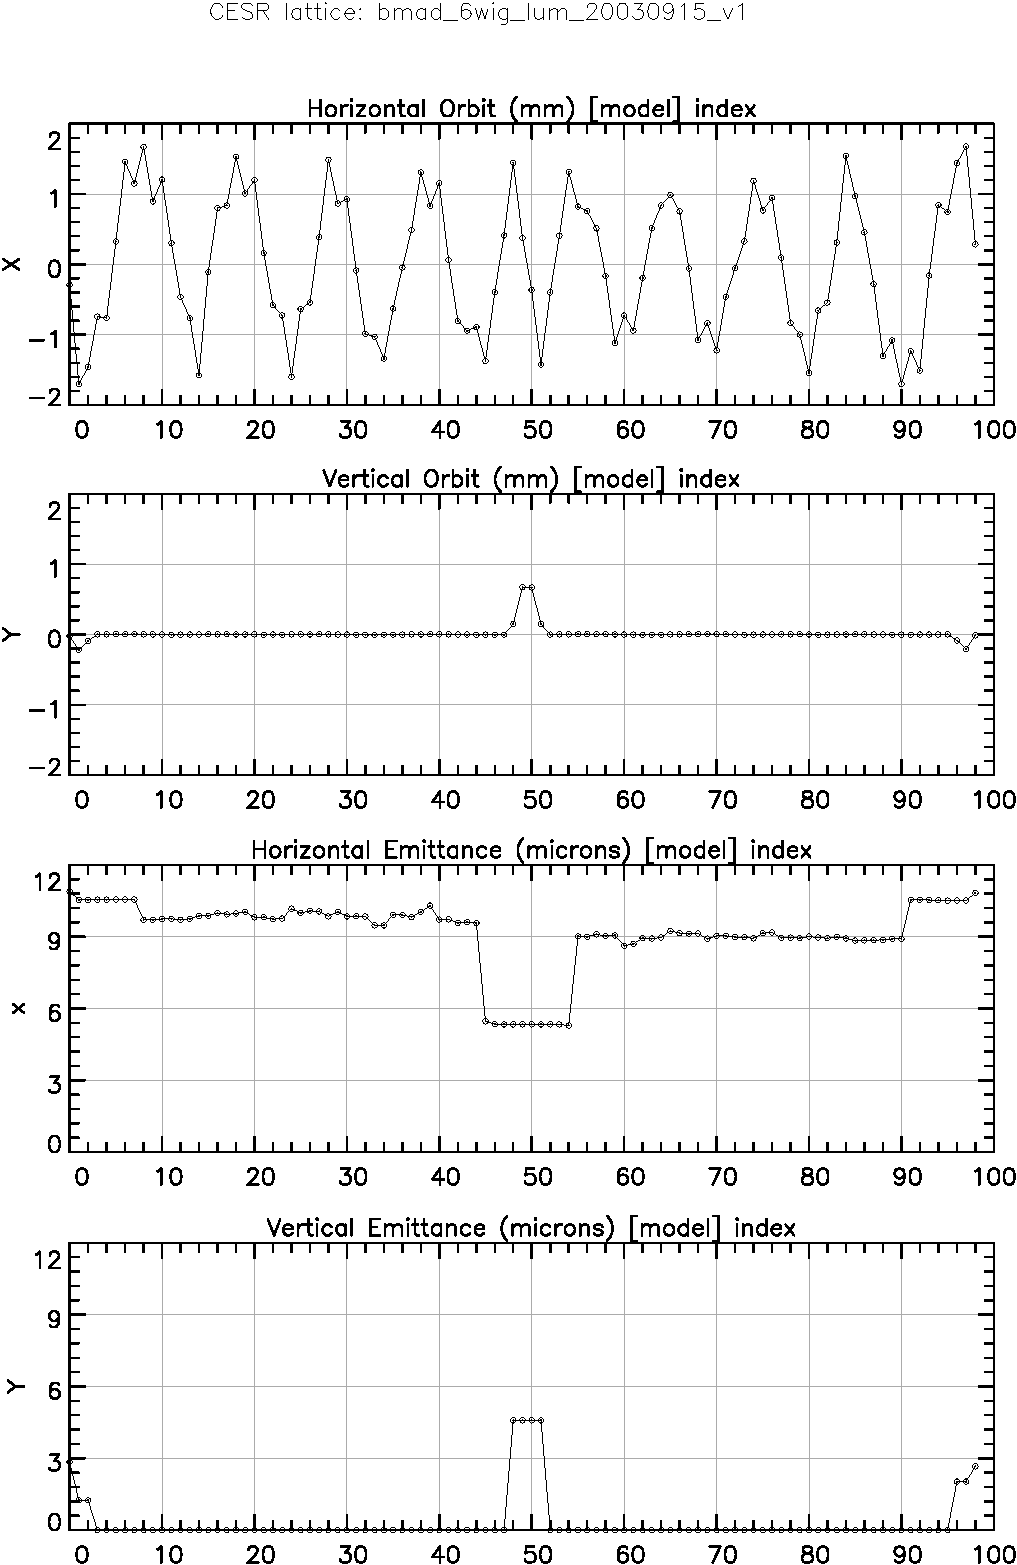
\includegraphics[width=5in]{plot-emittance.pdf}
  \caption{Custom data type: non-normalized emittance}
  \label{f:plot.emittance}
\end{figure}
